\documentclass[main.tex]{subfiles}
    \usepackage{amsmath}
    \usepackage{amsfonts}
    \usepackage{listings}
    \usepackage{graphicx}
    \graphicspath{ {./img/} } 
    \usepackage{array}
    \usepackage{multicol}

\begin{document}
\begin{enumerate}
	\item Wie viele Relationen auf einer endlichen Menge \( A \) mit \( n \) Elementen gibt es?

	      Lösung:
	      \begin{enumerate}
		      \item Denn für eine Relation müssen immer \( 2 \) Elemente aus einer Menge ausgewählt werden.
		            Da diese auch das gleiche sein können, gibt es für das erste \( n \) Möglichkeiten. Für das
		            \( 2. \) wieder \( n \).

		            Somit ergeben sich \( n^2 \) Paare. Für jedes dieser gibt es die Möglichkeit es in der
		            Relation zu enthalten, oder nicht. Dadurch ergibt sich eine binäre Auswahl pro Element.

		            Es gibt somit \( 2^{n^2} \) Möglichkeiten.
	      \end{enumerate}
	\item Gib für \( A = \{x, y, z\} \) Relationen an mit folgenden Eigenschaften:
	      \begin{enumerate}
		      \item Reflexiv, aber nicht symmetrisch
		      \item Weder symmetrisch noch antisymmetrisch
		      \item Antisymmetrisch, aber nicht asymmetrisch
		      \item Total, aber nicht transitiv
		      \item Symmetrisch und total
	      \end{enumerate}

	      Lösung:
	      \begin{enumerate}
		      \item \( R := \{ (x,x), (y,y), (z,z) \} \)
		      \item \( R := \{ (x,y), (y,z), (z,x) \} \)
		      \item \( R := \{ (x,x), (y,y), (z,z) \} \)
		      \item \( R := \{ (x,y), (y,z), (z,x), (y,y), (x,x), (z,z) \} \)
		      \item \( R := \{ (x,y), (y,z), (z,x), (y,x), (z,y), (x,z) \} \)
	      \end{enumerate}
	\item Hier sind alle Relationen auf der Menge \( A = \{ x, y \} \):

	      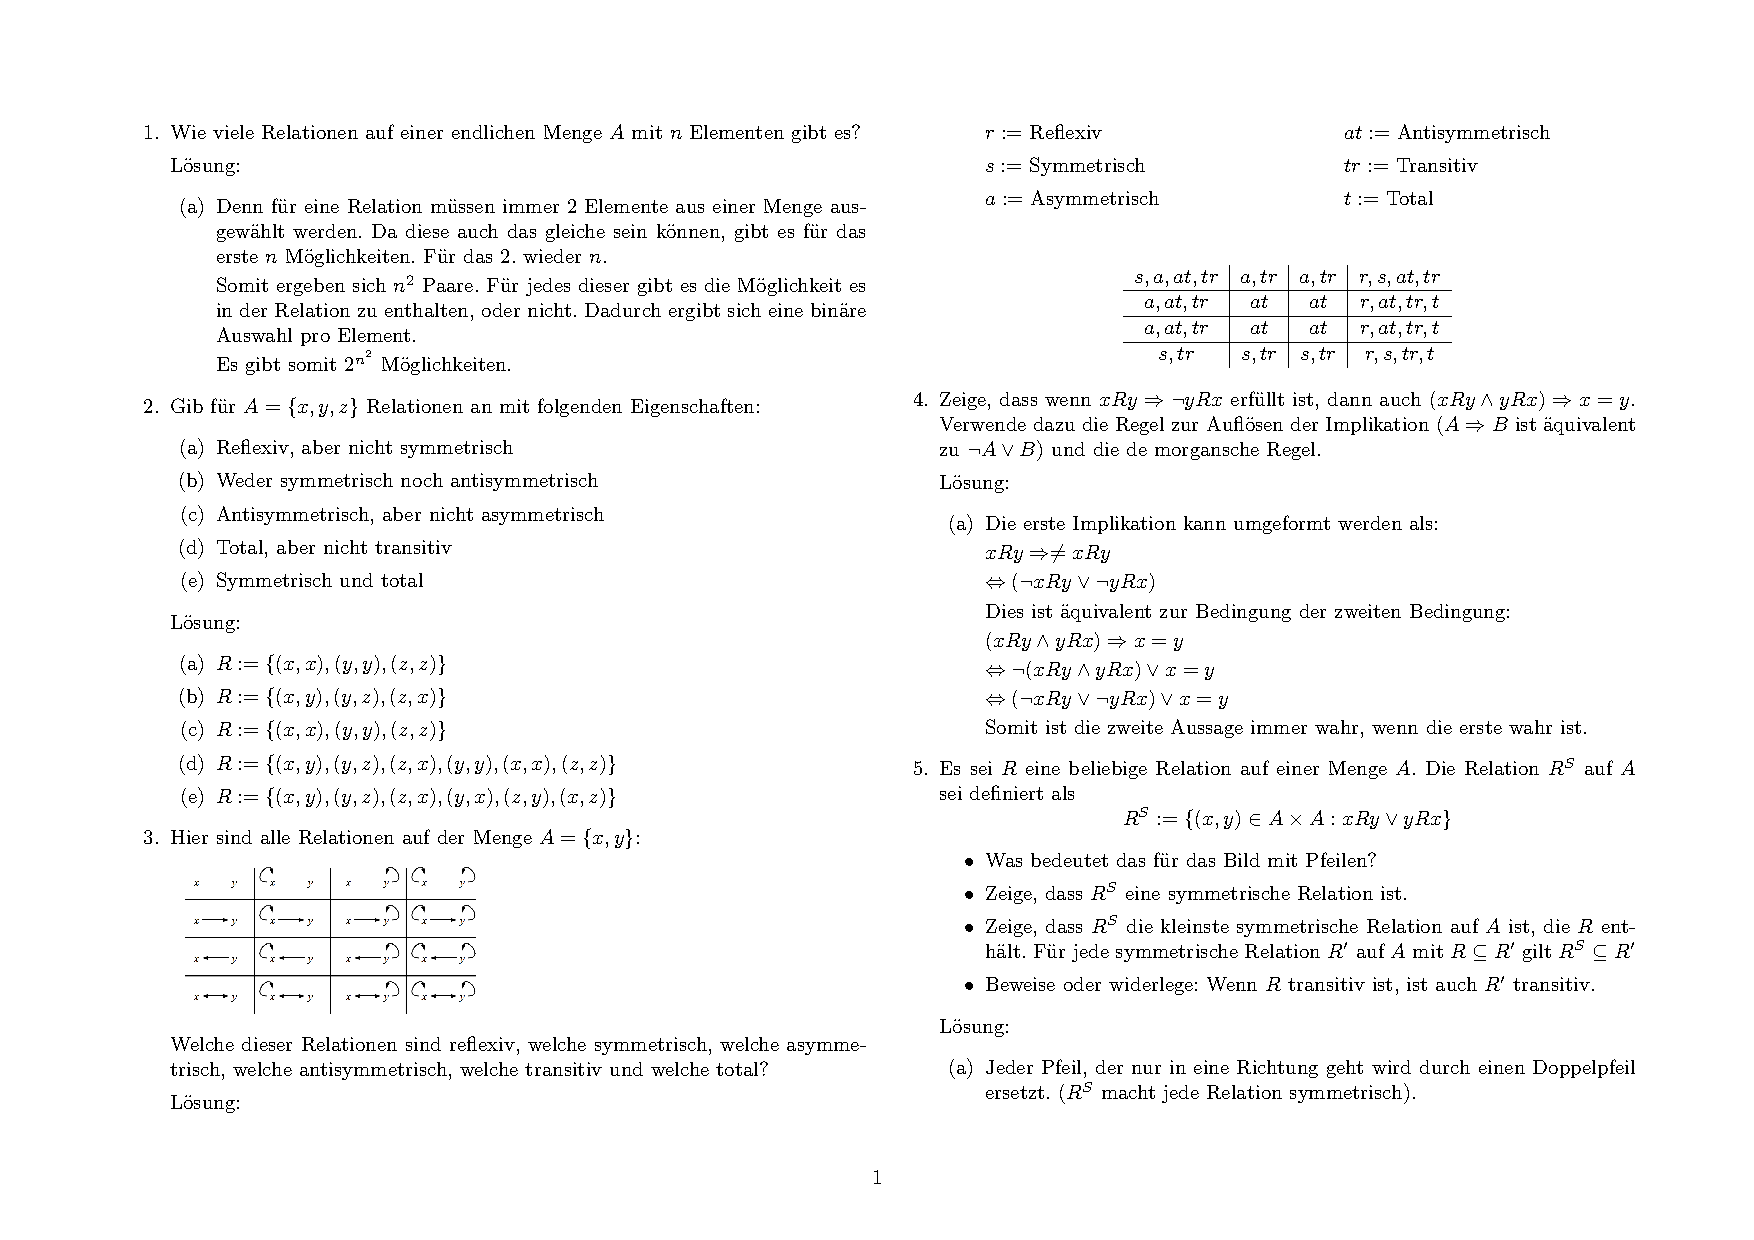
\includegraphics[scale=0.25]{relationen}

	      Welche dieser Relationen sind reflexiv, welche symmetrisch, welche asymmetrisch,
	      welche antisymmetrisch, welche transitiv und welche total?

	      Lösung:
	      \begin{multicols}{2}
		      \begin{itemize}
			      \item[] \( r := \) Reflexiv
			      \item[] \( s := \) Symmetrisch
			      \item[] \( a := \) Asymmetrisch
			      \item[] \( at :=  \) Antisymmetrisch
			      \item[] \( tr :=  \) Transitiv
			      \item[] \( t := \) Total
		      \end{itemize}
	      \end{multicols}
	      \[
		      \begin{array}{c|c|c|c}
			      s, a, at, tr & a, tr & a, tr & r, s, at, tr \\
			      \hline
			      a, at, tr    & at    & at    & r, at, tr, t \\
			      \hline
			      a, at, tr    & at    & at    & r, at, tr, t \\
			      \hline
			      s ,tr        & s, tr & s,tr  & r, s, tr, t  \\
		      \end{array}
	      \]
	\item
	      Zeige, dass wenn \( xRy \Rightarrow \neg yRx \) erfüllt ist, dann auch
	      \( (xRy \land yRx) \Rightarrow x = y \).
	      Verwende dazu die Regel zur Auflösen der Implikation (\( A \Rightarrow B  \) ist äquivalent
	      zu \( \neg A \lor B \)) und die de morgansche Regel.

	      Lösung:
	      \begin{enumerate}
		      \item  Die erste Implikation kann umgeformt werden als:

		            \( xRy \Rightarrow \neq xRy \)

		            \( \Leftrightarrow (\neg xRy \lor \neg yRx) \)


		            Dies ist äquivalent zur Bedingung der zweiten Bedingung:

		            \( (xRy \land yRx) \Rightarrow x = y \)

		            \( \Leftrightarrow \neg(xRy \land yRx) \lor x = y \)

		            \( \Leftrightarrow (\neg xRy \lor \neg yRx) \lor x = y \)

		            Somit ist die zweite Aussage immer wahr, wenn die erste wahr ist.
	      \end{enumerate}
	\item Es sei \( R \) eine beliebige Relation auf einer Menge \( A \).
	      Die Relation \( R^S \) auf \( A \) sei definiert als
	      \[ R^S := \{ (x,y) \in A \times A : xRy \lor yRx \} \]
	      \begin{itemize}
		      \item Was bedeutet das für das Bild mit Pfeilen?
		      \item Zeige, dass \( R^S \) eine symmetrische Relation ist.
		      \item Zeige, dass \( R^S \) die kleinste symmetrische Relation auf \( A \) ist,
		            die \( R \) enthält.
		            Für jede symmetrische Relation \( R' \) auf \( A \) mit \( R \subseteq R' \)  gilt
		            \( R^S \subseteq R' \)
		      \item Beweise oder widerlege: Wenn \( R \) transitiv ist, ist auch \( R' \) transitiv.
	      \end{itemize}

	      Lösung:
	      \begin{enumerate}
		      \item Jeder Pfeil, der nur in eine Richtung geht wird durch einen Doppelpfeil ersetzt.
		            (\( R^S \) macht jede Relation symmetrisch).
		      \item \( R^S \) ist symmetrisch, denn falls ein Paar \( (x,y) \in R^S \) muss entweder
		            \( xRy \lor yRx \) aus der Relation \( R \) gelten.

		            Somit muss auch das Paar \( (y,x) \in R^S \),
		            denn wenn beim vorherigen \( xRy \) war muss nun \( yRx \) oder umgekehrt sein.
		      \item
		      \item
	      \end{enumerate}
	\item Gibt es Relationen, die sowohl reflexiv, aus auch asymmetrisch sind?
	      (Vorsicht: genau hinsehen!)

	      Lösung:
	      \begin{enumerate}
		      \item Es gibt nur eine Relation, die reflexiv sowie asymmetrisch ist. Dies ist die Relation
		            auf der leeren Menge.
		            \[ A = \{ \} \]

		            Reflexivität:

		            \( \forall x \in A: xRx \), da \( A = \{\} \) ist dies der Fall.

		            Asymmetrie:

		            \( \forall x,y \in A: (xRy \land yRx) \Rightarrow x = y\)
		            Da \( A = \{\} \) ist die Prämisse immer falsch, wodurch die Implikation wahr wird.
	      \end{enumerate}
\end{enumerate}
\end{document}